%\begin{frame}{Upgrade plans: Run-3 and HL-LHC}
%    \begin{figure}
%        \centering
%        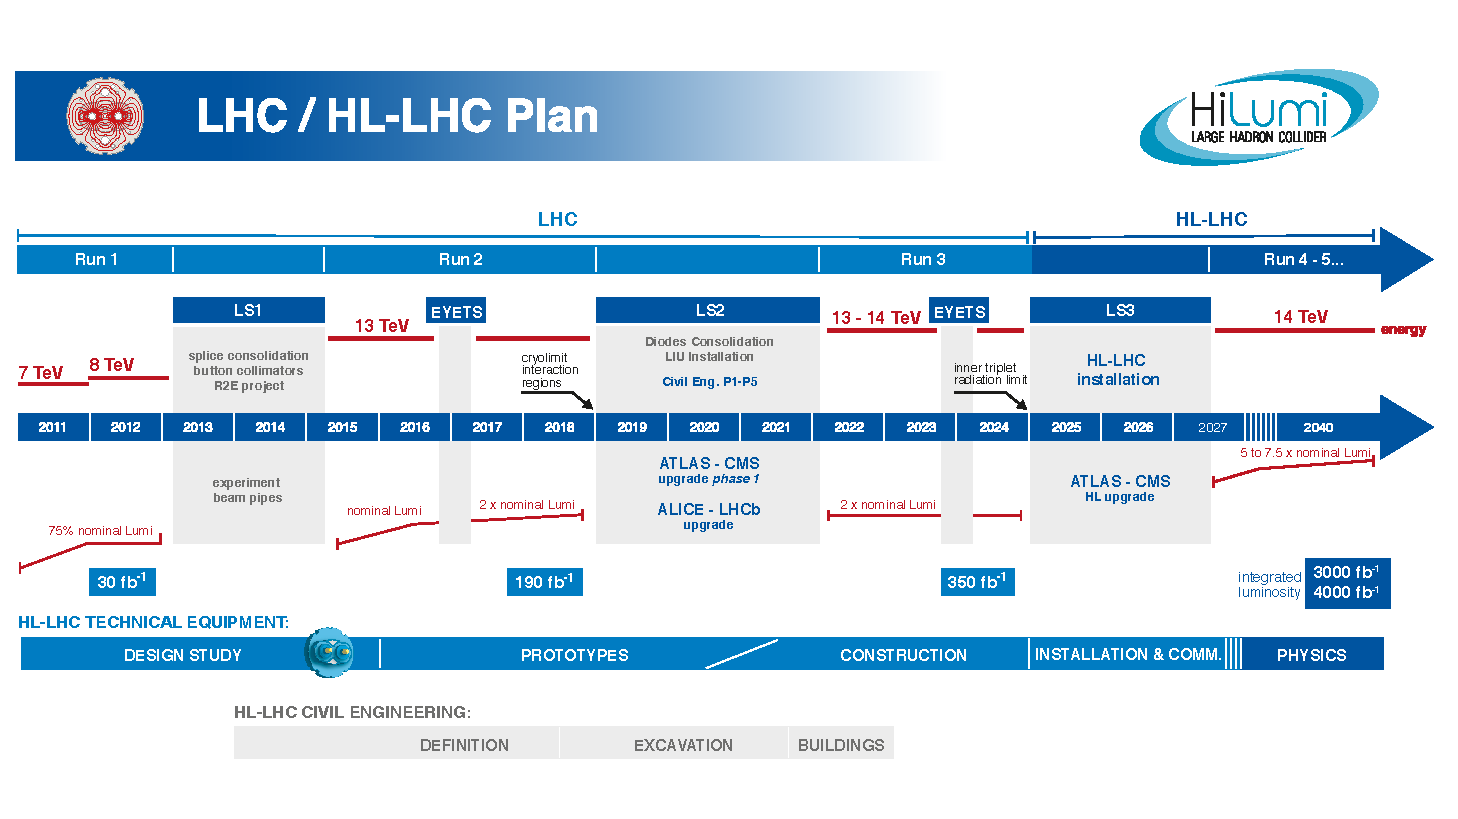
\includegraphics[width=0.6\textwidth]{Part2/Img/HL-LHC-plan-2021-1.pdf}
%    \end{figure}
%\begin{columns}
%\column{0.5\textwidth}  
%\begin{center}
%    \textbf{Run-3}
%\end{center}
%\begin{itemize}
%    \item $\sqrt{s}=$ 13.6 TeV
%    \item $\mathcal{L}_{int} \sim $ 300 fb$^{-1}$
%\end{itemize}
%\column{0.5\textwidth}  
%
%\begin{center}
%    \textbf{High-Luminosity LHC}
%\end{center}
%\begin{itemize}
%    \item $\sqrt{s}=$ 14 TeV
%    \item $\mathcal{L}_{int} \sim $  3000 fb$^{-1}$
%\end{itemize}
%
%\end{columns}
%\end{frame}


\subsection{Prospects at the end of Run-3}
\begin{frame}{Prospects at the end of Run-3}
\begin{textblock*}{5cm}(12cm,0.1cm) % {block width} (coords) 
   \textcolor{HHred}{\Large\textbf{my own work}}
\end{textblock*}
\begin{columns}
\column{0.6\textwidth}

\begin{itemize}
    \item \textbf{Run-2+Run-3}: $\mathcal{L}_{int} \sim $ 300 fb$^{-1}$, $\sqrt{s}$ = 13.6 TeV
    \begin{itemize}
        \item Detector upgrades: \textbf{no significant impact on HH$\to b\bar{b}\gamma\gamma$}
    \end{itemize}
\end{itemize}
\onslide<2->{
\begin{itemize}
    \item $\frac{\sigma_{HH}}{\sigma_{HH}^{SM}}$ limit: \textcolor{HHred}{\textbf{3.3}} (\textcolor{cadmiumorange}{\textbf{1.6$\times$ imp.}} w.r.t 139 fb$^{-1}$)
\end{itemize}
\begin{table}
    \centering
    \begin{tabular}{lcc}
    \hline\hline
        Scenario & 1$\sigma$ CI & 2$\sigma$ CI  \\
        \hline
        \textcolor{blue}{Run-2} & \textcolor{blue}{[-1.3, 6.4]} & \textcolor{blue}{[-2.9, 8]} \\
        Run-2+Run-3 & \textbf{[-0.7, 5.6]} & \textbf{[-1.9, 7]} \\
        \hline\hline
    \end{tabular}
\end{table}
}
\onslide<3->{

\underline{Potential improvements}:
\begin{itemize}
    \item \textbf{DNN categorization}: \textcolor{HHred}{\textbf{$\sim$10\%}}
    \item $m_{b \bar{b}}$ imp. with \textbf{kinematic fit}: \textcolor{HHred}{\textbf{2-5\%}}
    \item \textbf{Photon identification}: \textcolor{HHred}{\textbf{7\%}} (next part)
\end{itemize}
}
\column{0.4\textwidth}

\visible<2->{
\begin{figure}
    \centering
    \fcolorbox{HHred}{HHwhite2}{
    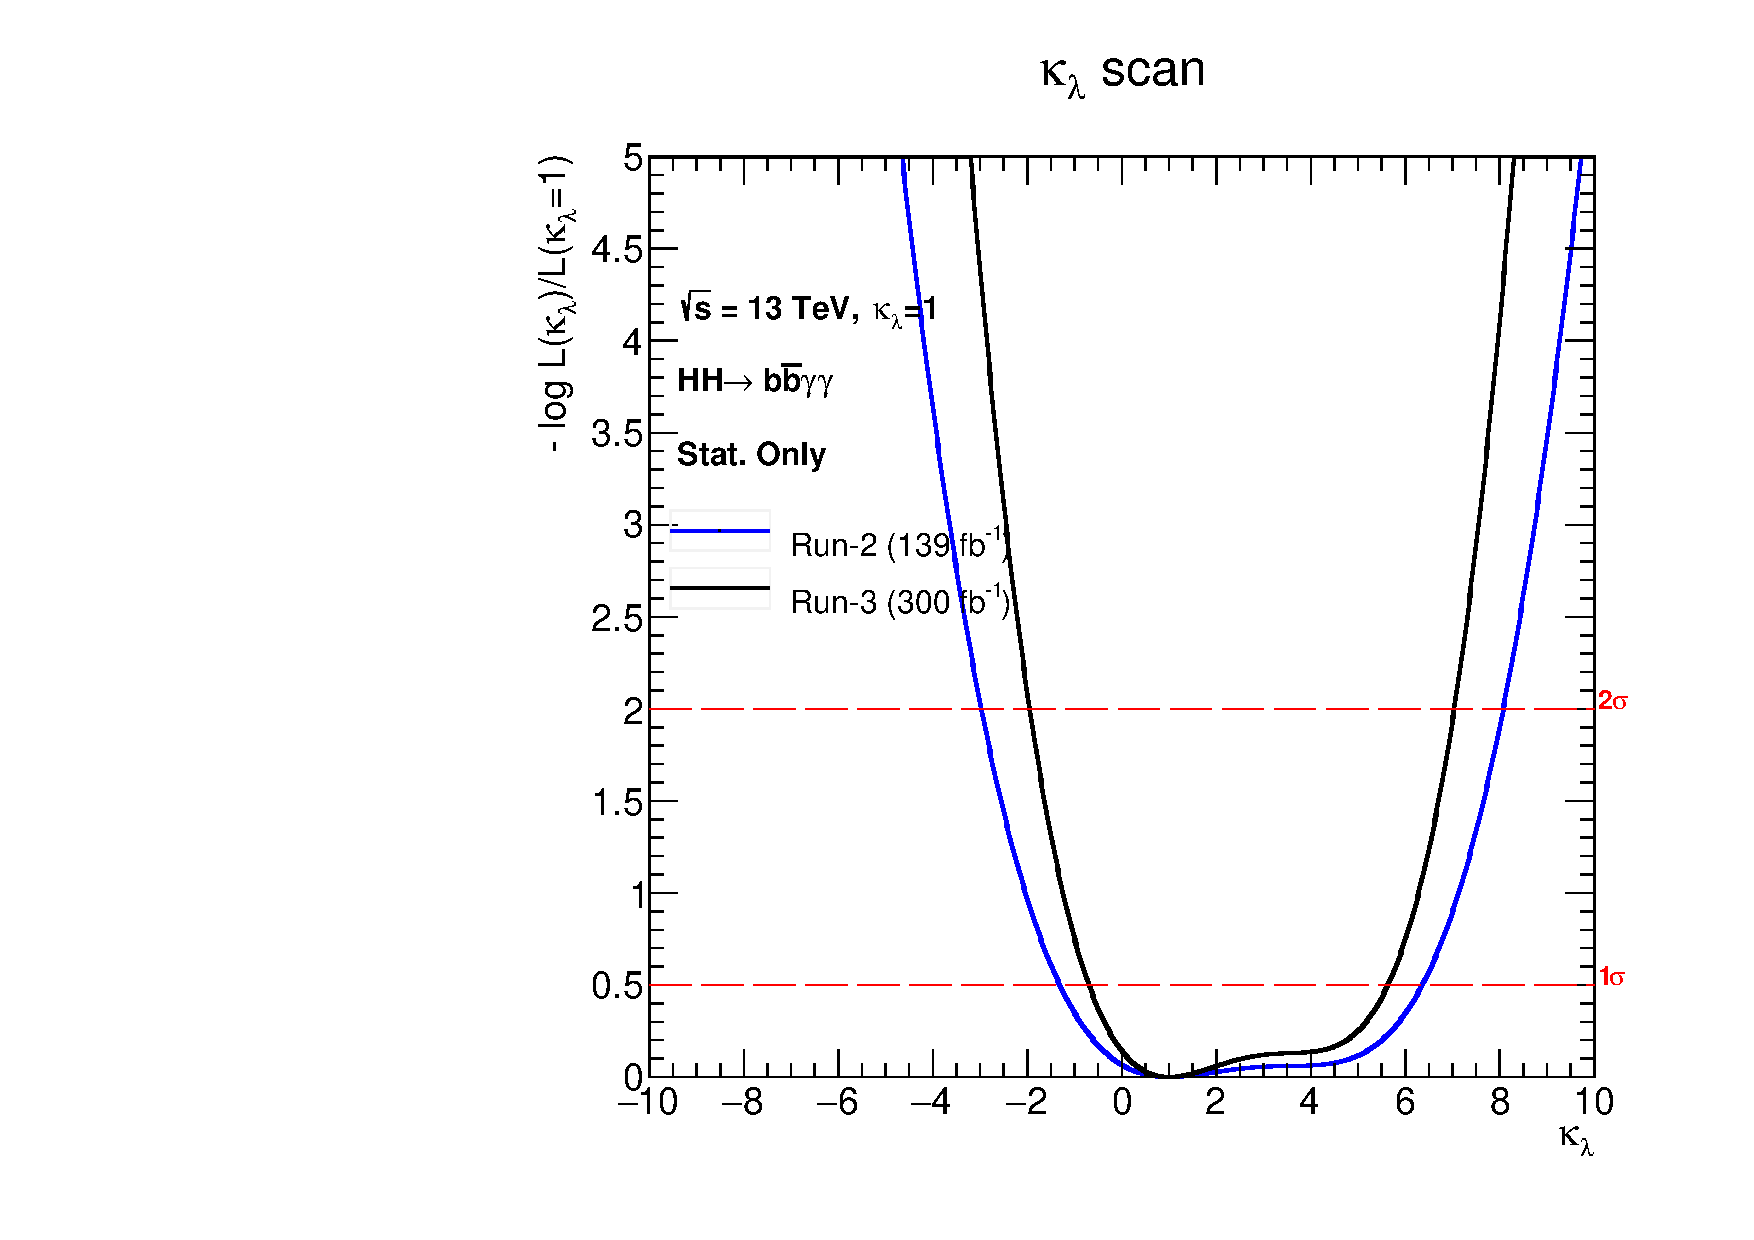
\includegraphics[width=1\textwidth]{Part4/Img/likelihood_subplot_Run3.pdf}
    }
\end{figure}
}
\end{columns}
\end{frame}

\subsection{Prospects at HL-LHC}
\begin{frame}{Prospects at HL-LHC}
\begin{textblock*}{5cm}(12cm,0.1cm) % {block width} (coords) 
   \textcolor{HHred}{\Large\textbf{my own work}}
\end{textblock*}
\begin{columns}
\column{0.4\textwidth}

\begin{figure}
    \begin{overprint}
    %\onslide<1>\centering\fcolorbox{HHturquoise_d}{HHwhite2}{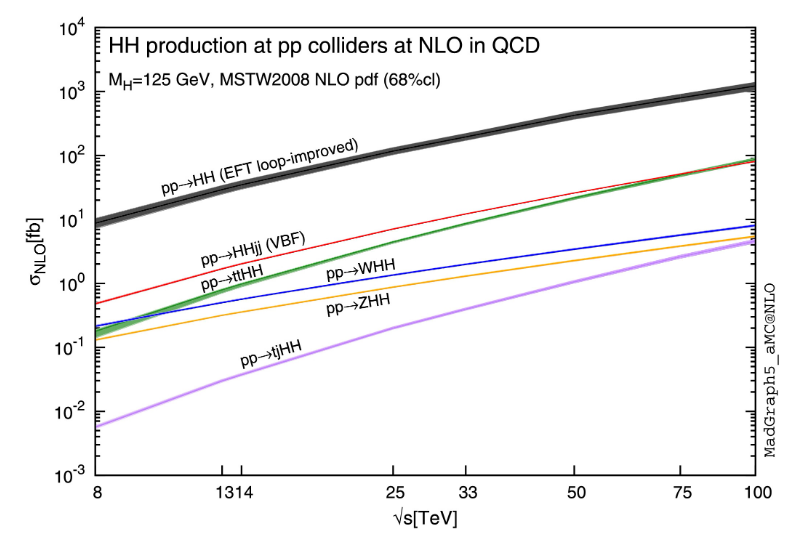
\includegraphics[width=1\textwidth]{Part1/Img/HH_XSec_as_S.png}}
    \onslide<2->\centering\fcolorbox{HHred}{HHwhite2}{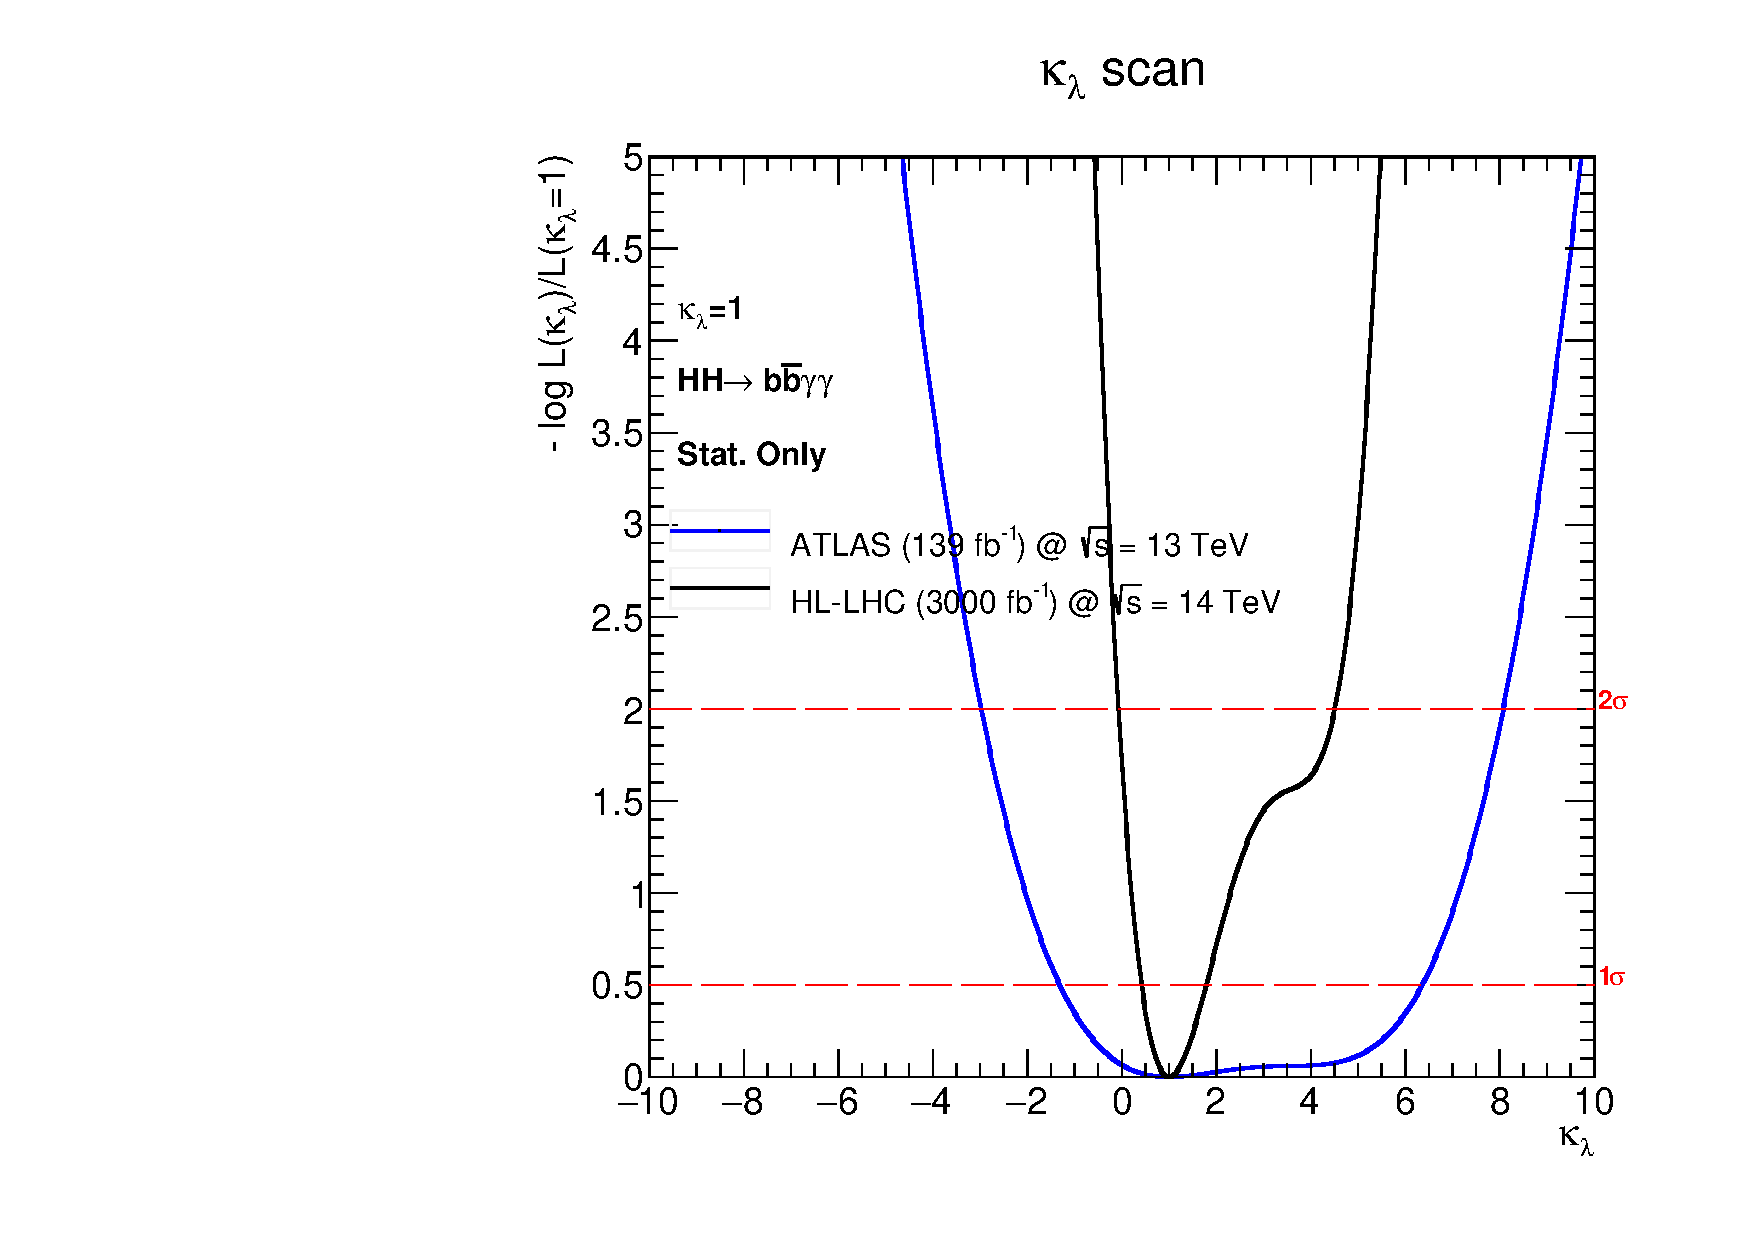
\includegraphics[width=1\textwidth]{Part4/Img/likelihood_subplot_14TeV.pdf}}
   \end{overprint}
\end{figure}


\column{0.6\textwidth}
\begin{itemize}
    \item \textbf{HL-LHC: \textcolor{HHturquoise_d}{$\sim$3000 fb$^{-1}$} at \textcolor{HHturquoise_d}{14 TeV}}
    \onslide<2->{
    \item Detector upgrades: \textbf{mitigate higher pileup effects} 
    \item European strategy: extrapolation from 36 fb$^{-1}$
    }
\end{itemize}
\onslide<2->{
\begin{table}[]
    \centering
    \begin{tabular}{lcc}
        \hline\hline
        Scenario & 1$\sigma$ CI & 2$\sigma$ CI  \\
        \hline
        \textcolor{blue}{European strategy} & \textcolor{blue}{[-0.1, 2.4]} & \textcolor{blue}{[-1.1, 8.1]} \\
        My Extra. to HL-LHC & \textbf{[0.4, 1.8]} & \textbf{[-0.1, 4.4]} \\
        \hline\hline
    \end{tabular}
\end{table}
}

\end{columns}    
\end{frame}

\begin{frame}{Prospects at HL-LHC}
\begin{textblock*}{5cm}(12cm,0.1cm) % {block width} (coords) 
   \textcolor{HHred}{\Large\textbf{my own work}}
\end{textblock*}
\begin{columns}
\column{0.4\textwidth}

\begin{figure}
  \centering
  \fcolorbox{HHturquoise_d}{HHwhite2}{
   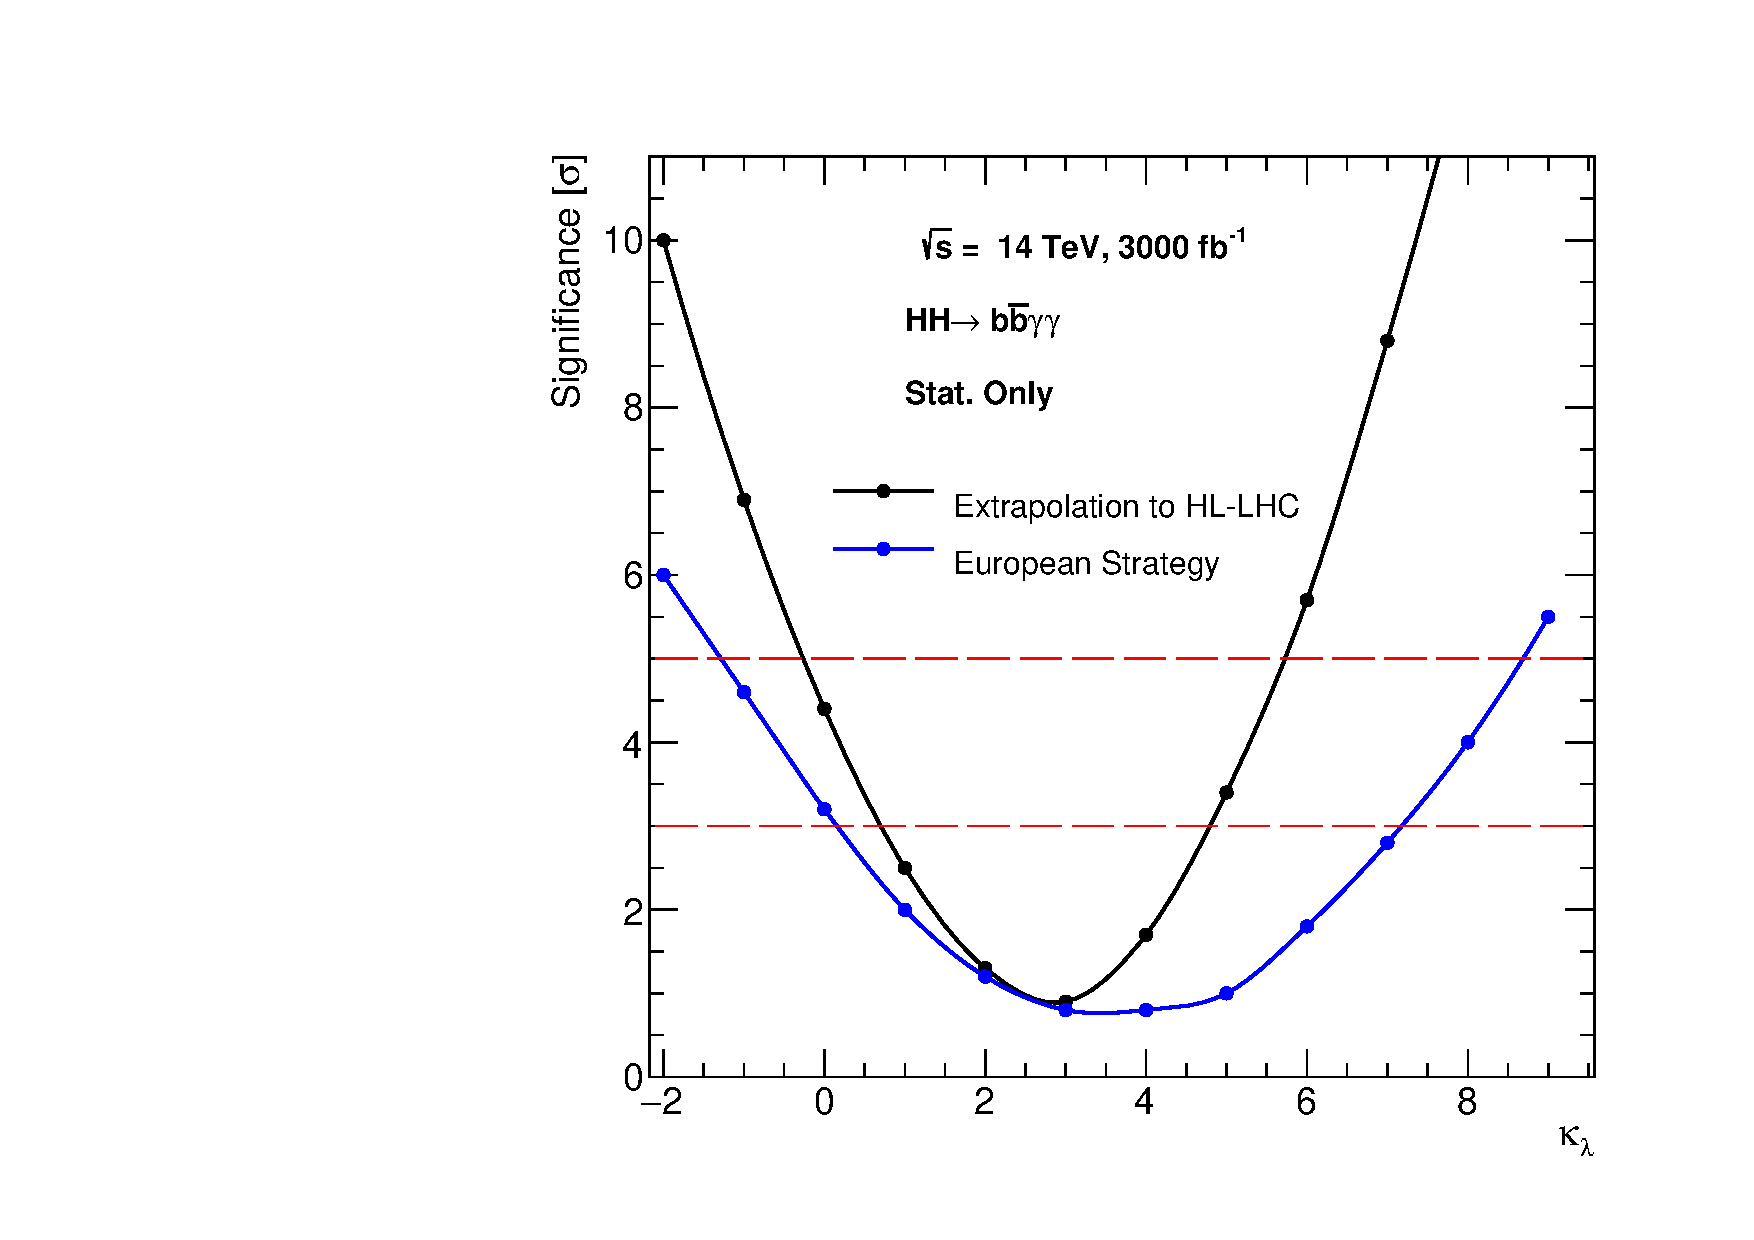
\includegraphics[width=1\textwidth]{Part4/Img/sig.pdf}
   }
\end{figure}


\column{0.6\textwidth}
\begin{itemize}
    \item \textbf{HL-LHC: \textcolor{HHturquoise_d}{$\sim$3000 fb$^{-1}$} at \textcolor{HHturquoise_d}{14 TeV}}
    \item Detector upgrades: \textbf{mitigate higher pileup effects} 
    \item European strategy: extrapolation from 36 fb$^{-1}$
\end{itemize}

\begin{table}[]
    \centering
    \begin{tabular}{lc}
        \hline\hline
        Scenario & Significance [$\sigma$]  \\
        \hline
        \textcolor{blue}{European strategy} & \textcolor{blue}{2.1} \\
        My Extra. to HL-LHC & \textbf{2.5} \\
        \hline\hline
    \end{tabular}
\end{table}

\begin{center}
    \textbf{\textcolor{HHturquoise_d}{Similar performances for SM} } \\
    \textbf{\textcolor{HHred}{Large gain at high $\kappa_{\lambda}$}}
\end{center}

\end{columns}  
\end{frame}